
%!TEX ROOT=ctutest.tex

\chapter{Rešerše}


\section{Podlahové topení}

U podlahového vytápění dochází k přenosu tepla do vytápěného prostoru převážně sáláním. Což má za následek, že se od sálající plochy ohřívají plochy osálané a teprve od sálajících a osálaných ploch se ohřívá okolní vzduch (druhá konvenkční složka z celkového tepelného toku). Naproti tomu při přenosu tepla pomocí tradičních radiátorů dochází k přenosu pomocí proudění (konvekční složka). 
Teplota otopné plochy je poměrně nízká pohybuje se mezi 25 až 34~°C u podlahového vytápění a tedy i teplota teplonosné látky je nízká (otopná plocha je zahřívaná buď teplou vodou, teplým vzduchem nebo elektricky). Proto je tento typ vytápění vhodné využít při zapojení s nízkoteplotním zdrojem, jako jsou tepelná čerpadla, kondenzační kotle či solární panely.

Důležitým parametrem pro příjemný pobyt v místnosti je prostorové rozložení teploty, jak ve vertikální tak horizontální rovině. Na vertikální rozložení teplot ve vytápěné místnosti je způsobeno nerovnoměrným přívodem tepla a nerovnoměrným ochlazování jednotlivých stěn místnosti. Vertikální nerovnoměrnost teplot je tím větší, čím vyšší je povrchová teplota otopné plochy. Vzhledem k tomu, že teplota u podlahové vytápění je povrchová teplota otopné vody ze všech druhů velkoplošného vytápění (podlahové, stropní, stěnové) nejnižší, je vertikální rozložení teplot skoro ideální, viz obrázek \ref{fig:vertikalni-prubehy-teplot-pro-ruzne-druhy-vytapeni}a. Optimální vytápění by mělo zajistit, aby v oblasti hlavy stojícího člověka byla teplota minimálně o 2 °C nižší než je v úrovni kotníků. Takovému ideálnímu průběhu teplot odpovídá obrázek \ref{fig:vertikalni-prubehy-teplot-pro-ruzne-druhy-vytapeni}b. Dále jsou na obrázku  \ref{fig:vertikalni-prubehy-teplot-pro-ruzne-druhy-vytapeni} jsou další druhy vytápění s vertikálními průběhy teplot. Na obrázku \ref{fig:porovnani-rozlozeni-teplot} je prostorové porovnání teplot podlahové vytápění a vytápění při využití radiátorů s~vyznačenými oblastmi teplot.


\begin{figure}[h]

\centering
\begin{picture}(370,150)
\put(0,0){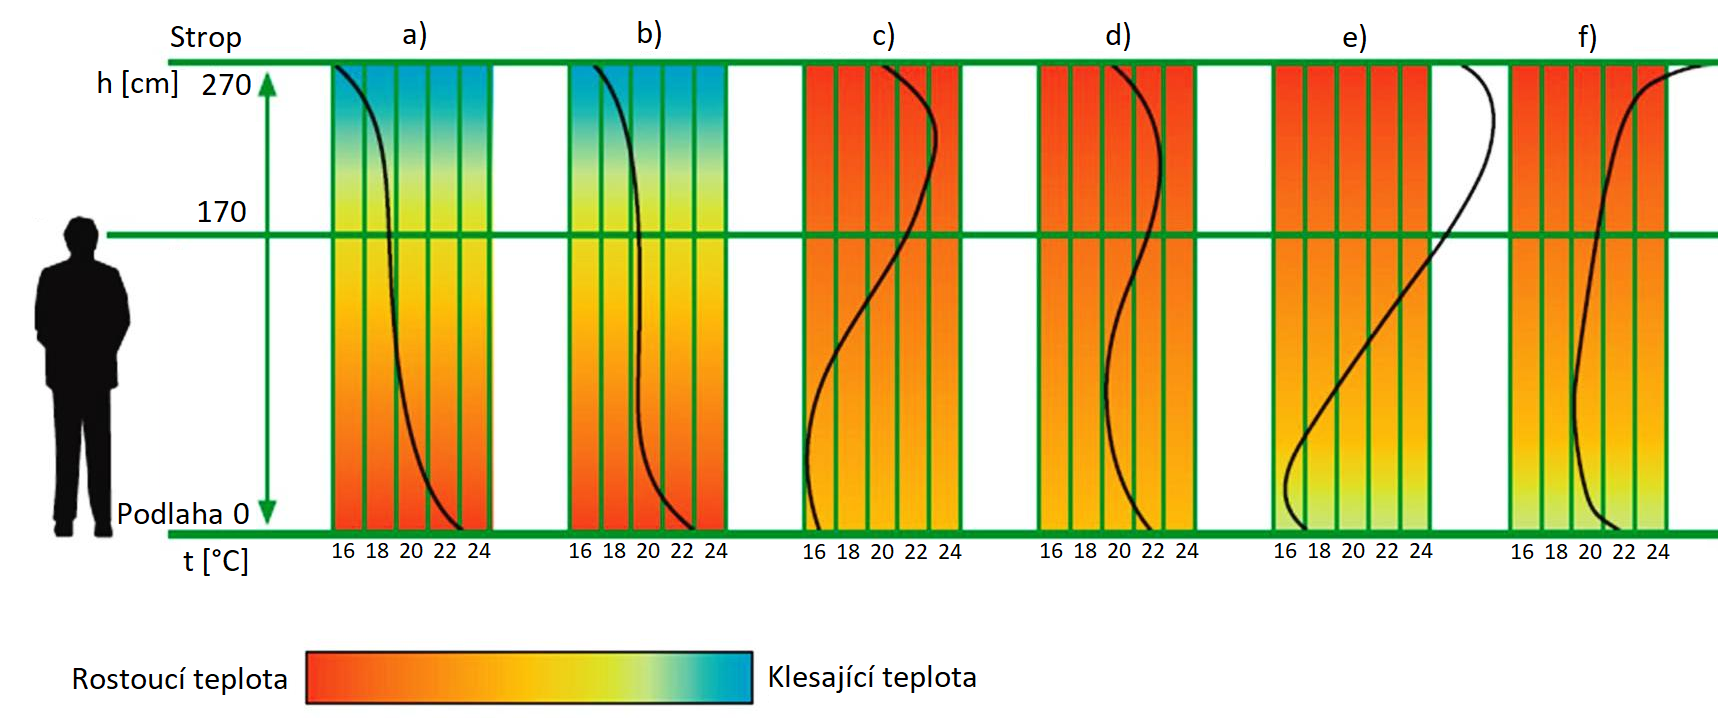
\includegraphics[width=\textwidth]{images/vertikalni-prubehy-teplot-pro-ruzne-druhy-vytapeni.png}}
\put(5,6){\scriptsize \sffamily Rostoucí teplota}
\put(161,6){\scriptsize \sffamily Klesající teplota}
\put(19,31){\scriptsize \sffamily t[°C]}
\put(15,132){\scriptsize \sffamily h[cm]}
\put(22,41){\fontsize{6}{6} \sffamily Podlaha}
\put(22,141){\fontsize{6}{6} \sffamily Strop}
\put(50,41){\scriptsize \sffamily 0}
\put(40,104){\scriptsize \sffamily 170}
\put(40,132){\scriptsize \sffamily 270}

\put(84,143){\scriptsize \sffamily a)}
\put(67,33){\fontsize{5}{5} \sffamily 16}
\put(74,33){\fontsize{5}{5} \sffamily 18}
\put(81,33){\fontsize{5}{5} \sffamily 20}
\put(88,33){\fontsize{5}{5} \sffamily 22}
\put(95,33){\fontsize{5}{5} \sffamily 24}

\put(134,143){\scriptsize \sffamily b)}
\put(117,33){\fontsize{5}{5} \sffamily 16}
\put(124,33){\fontsize{5}{5} \sffamily 18}
\put(131,33){\fontsize{5}{5} \sffamily 20}
\put(138,33){\fontsize{5}{5} \sffamily 22}
\put(145,33){\fontsize{5}{5} \sffamily 24}

\put(184,143){\scriptsize \sffamily c)}
\put(167,33){\fontsize{5}{5} \sffamily 16}
\put(174,33){\fontsize{5}{5} \sffamily 18}
\put(181,33){\fontsize{5}{5} \sffamily 20}
\put(188,33){\fontsize{5}{5} \sffamily 22}
\put(195,33){\fontsize{5}{5} \sffamily 24}

\put(234,143){\scriptsize \sffamily d)}
\put(217,33){\fontsize{5}{5} \sffamily 16}
\put(224,33){\fontsize{5}{5} \sffamily 18}
\put(231,33){\fontsize{5}{5} \sffamily 20}
\put(238,33){\fontsize{5}{5} \sffamily 22}
\put(245,33){\fontsize{5}{5} \sffamily 24}

\put(284,143){\scriptsize \sffamily e)}
\put(267,33){\fontsize{5}{5} \sffamily 16}
\put(274,33){\fontsize{5}{5} \sffamily 18}
\put(281,33){\fontsize{5}{5} \sffamily 20}
\put(288,33){\fontsize{5}{5} \sffamily 22}
\put(295,33){\fontsize{5}{5} \sffamily 24}

\put(334,143){\scriptsize \sffamily f)}
\put(317,33){\fontsize{5}{5} \sffamily 16}
\put(324,33){\fontsize{5}{5} \sffamily 18}
\put(331,33){\fontsize{5}{5} \sffamily 20}
\put(338,33){\fontsize{5}{5} \sffamily 22}
\put(345,33){\fontsize{5}{5} \sffamily 24}
\end{picture}
	 \caption{Vertikální průběh teploty vzduchu ve vytápěné místnosti při různém způsobu vytápění. Upraveno z \cite{vertikalni-prubehy-teplot-pro-ruzne-druhy-vytapeni}. \\ a) Ideální požadovaný průběh, b) Podlahové vytápění, c) Vytápění radiátory (vnitřní stěna), d) Vytápění radiátory (venkovní stěna), e) Teplovzdušné vytápění (podlahové konvektory), f) Stropní vytápění }
	 \label{fig:vertikalni-prubehy-teplot-pro-ruzne-druhy-vytapeni}
\end{figure}

\hspace{5mm}

  \begin{figure}[H]
     \subfloat[Rozložení teplot při použití podlahové topení.\label{fig:rozlozeni-teplot-podlahove-vytapeni}]{
       \begin{overpic}[width=0.5\textwidth]{images/rozlozeni-teplot-podlahove-vytapeni.png}
         \put(20,10){\scriptsize \sffamily 22 °C}
         \put(65,50){\scriptsize \sffamily 20 °C}
         \put(8,115){\scriptsize \sffamily 17 °C}
         \put(155,90){\scriptsize \sffamily 18 °C}
       \end{overpic}
     }
     \subfloat[Rozložení teplot při použití radiátorů. \label{fig:rozlozeni-teplot-radiatory}]{
       \begin{overpic}[width=0.5\textwidth]{images/rozlozeni-teplot-radiatory.png}
         \put(20,10){\scriptsize \sffamily 14 °C}
         \put(100,15){\scriptsize \sffamily 33 °C}
         \put(133,37){\scriptsize \sffamily 37 °C}
         \put(32,50){\scriptsize \sffamily 22 °C}
         \put(113,77){\scriptsize \sffamily 30 °C}
         \put(20,87){\scriptsize \sffamily 19 °C}
         \put(160,95){\scriptsize \sffamily 20 °C}
         \put(42,117){\scriptsize \sffamily 23 °C}
       \end{overpic}
     }
     \caption{Porovnání rozložení teplot při použití podlahové topení a radiátorů. Upraveno z \cite{rozlozeni-teplot-podlahove-vytapeni-a-radiatory}.}\label{fig:porovnani-rozlozeni-teplot}
   \end{figure}
   


\subsubsection{Výhody}

\begin{itemize}
  \item Je vhodné zejména tam, kde je nízkoteplotní zdroj tepla (tepelné čerpadlo, kondenzační kotel, solární panely, …).
  \item Větší užitný prostor (místo nezabírají otopná tělesa).
  \item Cirkulace vzduchu je nižší oproti radiátorům, proto je víření prachu v~místnosti menší.
  \item Téměř rovnoměrná teplota místnosti.
\end{itemize}

\subsubsection{Nevýhody}

\begin{itemize}
  \item Zvýšené náklady na realizaci.
  \item Nezbytná pečlivá montáž a stavební dozor.
  \item Vyšší tepelná setrvačnost otopné soustavy.
  \item Vyšší nároky na řízení podlahové otopné plochy (zejména hlídání maximální vstupní otopné vody).
\end{itemize}


\section{Zónová regulace vytápění}

Význam zónové regulace spočívá v systému umožňující individuální vytápění v~jednotlivých místnostech (každá místnost nebo spojení více místností označuje zónu) na požadovanou teplotu.  Základ zónové regulace je centrální řídicí jednotka, která přijímá data od jednotlivých místností (zejména jejich aktuální teplotu) a dává povely na zařízení, které ovládá (otevírání/zavírání pohonů u jednotlivých topných okruhů apod.). Přístup k řídicí jednotce je nejčastěji pomocí displeje, webového rozhraní nebo jejich kombinace. V řídicí jednotce se dá celý systém vytápění nastavit (nastavení časových a teplotních programů pro jednotlivé zóny a mnohé další). 

Zónové systémy vytápění se rozdělují na dvě hlavní skupiny. První tvoří zónové systémy propojené pomocí vodičů a druhou skupinu tvoří bezdrátová technologie propojující centrální řídicí jednotku a jednotlivé zóny. 

Hlavní částí zónového systému je centrální řídící jednotka. Mezi další komponenty patří, nástěnné snímače vnitřní teploty, snímač venkovní teploty, termoelektrické pohony, elektronické regulátory otopných těles, reléová spínací jednotka. Mezi komponenty, které přispívají ke komfortu zónové regulace jako senzor intenzity slunečního záření, senzor rychlosti větru, různé spínací jednotky, jednotky pro ovládání žaluzií, moduly pro dálkové ovládání pomocí GSM a další.
\subsection{Principy zónové regulace}
Jak již bylo řečeno, základem celého systému je centrální řídicí jednotka. Další důležitou komponentou je zónový regulátor, který slouží pro ovládání komponent, které jsou k zónovému regulátoru připojeny. Mezi hlavní komponenty, který zónový regulátor ovládá jsou termoelektrické pohony. Termoelektrický pohon je podobný termostatické hlavici, která se nasazuje na radiátorový ventil, ale je jej možné ovládat elektrickým napětím. Samotná regulace vytápění probíhá tak, že řídicí jednotka je propojena se zónovým regulátorem. K~zónovému regulátoru jsou připojeny jednotlivé nástěnné snímače  prostorové teploty a termoelektrické pohony, které jsou nasazeny na termostatický ventilech otopných okruhů/těles. V centrální jednotce jsou nastaveny časové programy (různé požadované teploty pro různé časové úseky). Centrální jednotka posílá do zónového regulátoru požadované teploty pro všechny zóny. Tyto  teploty jsou v zónovém regulátoru porovnávány s aktuálními prostorovými teplotami měřenými nástěnnými jednotkami. V případě, že je prostorová teplota příslušné zóny nižší než požadovaná teplota (nastavená v centrální jednotce), ovládá zónový regulátor odpovídající pohon, který otevírá/zavírá daný ventil a umožňuje proudění otopné vody do topného okruhu/tělesa, čím dochází ke změně teploty v místnosti. Pokud je připojen například kotel, je pak hořák kotle ovládán při požadavku vytápění v jakékoliv místnosti. Princip zónové regulace je zobrazen na obrázku \ref{fig:obecny-princip-zonove-regulace}.

Další možné zapojení může být takové, že jednotlivé nástěnné snímače prostorové teploty jsou přímo propojeny s centrální jednotkou, která následně podle časového programu posílá zónovému regulátoru požadavky na ovládání jednotlivých pohonů. 

Mezi další ovládána zařízení při regulace vytápění mohou být čerpadla, směšovací ventily zejména pro podlahové vytápění, kde je nutné udržovat teplotu otopné vody v daných mezích.

\begin{figure}[H]
    \centering
    \def\svgwidth{\columnwidth}
    \input{images/svg/obecny-princip-zonove-regulace.pdf_tex}
    \caption{ Obecný princip zónové podlahové regulace topení.}
    \label{fig:obecny-princip-zonove-regulace}
\end{figure}




\subsection{Dostupné komerční řešení zónové regulace podlahového vytápění}

Optimální systém pro otopnou soustavu, kterou hodlám řídit z obrázku \ref{fig:otopna-soustava-rez-domu} se skládá z řízení ovládání kotle, spínání čerpadel v případě zatopení v krbech a~následnou indikaci uživateli, jak moc je zásobník otopné vody natopen, dále z jednotlivých topných okruhů (12 pohonů pro 9 zón) a čerpadla podlahového topení. Pro zónovou regulaci se používá pouze patro.

\subsection{Elektrobock}
Česká firma Elektrobock nabízí bezdrátové řešení pro řízení podlahové topení. Systém řízení je zastřešené pod aplikaci PocketHome. Jednotlivé zařízení systému mohou fungovat samostatně bez nebo s centrální řídicí jednotkou. Tato centrální jednotka je zastřešené pod aplikaci PocketHome. Řídicí systém se skládá z centrální jednotky, nástěnných snímačů prostorové teploty pro jednotlivé místnosti a zónového regulátoru pro ovládání jednotlivých topných okruhů (celkově je možné ovládat 9 zón) a oběhového čerpadla, dále je k dispozici zařízení pro zapínání/vypínání kotle nebo komunikace pomocí protokolu OpenTherm. Na obrázku \ref{fig:elektrobock-pocket-home} jsou zobrazeny jednotlivé zařízení systému. Jistou nevýhodou může být bezdrátová komunikace na frekvenci 433,92 MHz, v případě delší vzdálenosti a především umístění na jiném patře centrální jednotky a lokální termostatů, zónového regulátoru může docházet k problémům s komunikací, zejména pokud se jedná o zástavbu z železobetonu, kde odrazivost a neprůchodnost signálu je poměrně značná. Jednotlivé prvky mohou pracovat samostatně bez centrální jednotky, na druhou stranu se tímto ztrácí přehled o celém systému a komfortu nastavování z jednoho místa. Systém se může nastavovat pomocí PC (systém Windows) nebo pomocí chytrého telefonu/tabletu (systém Android, iOS). Systém počítá s jedním zdrojem tepla, tedy kotlem (elektrickým, plynovým, automatickým), neuvažuje se s otopnou soustavu, kde je začleněn např. krb s tepelným výměníkem, jak z pohledu řízení čerpadel,tak i případnou indikaci o stavu natopení zásobníku s otopnou vodou. Další otázkou je využíti tohoto řídícího systému při použití centrální zásobníku na otopnou vodou, zejména při použití nízko teplotních zdrojů. Kde distribuce otopné vody pochází primárně z tohoto zásobníku, je nutné sledovat teplotu  a na základě toho spínat kotel pro dobíjení, případně jiných zdrojů tepla. Problém bezdrátového bateriového řešení je nutná výměna baterií po určité době.


\begin{figure}[H]

\centering
\begin{picture}(370,226)
\put(0,0){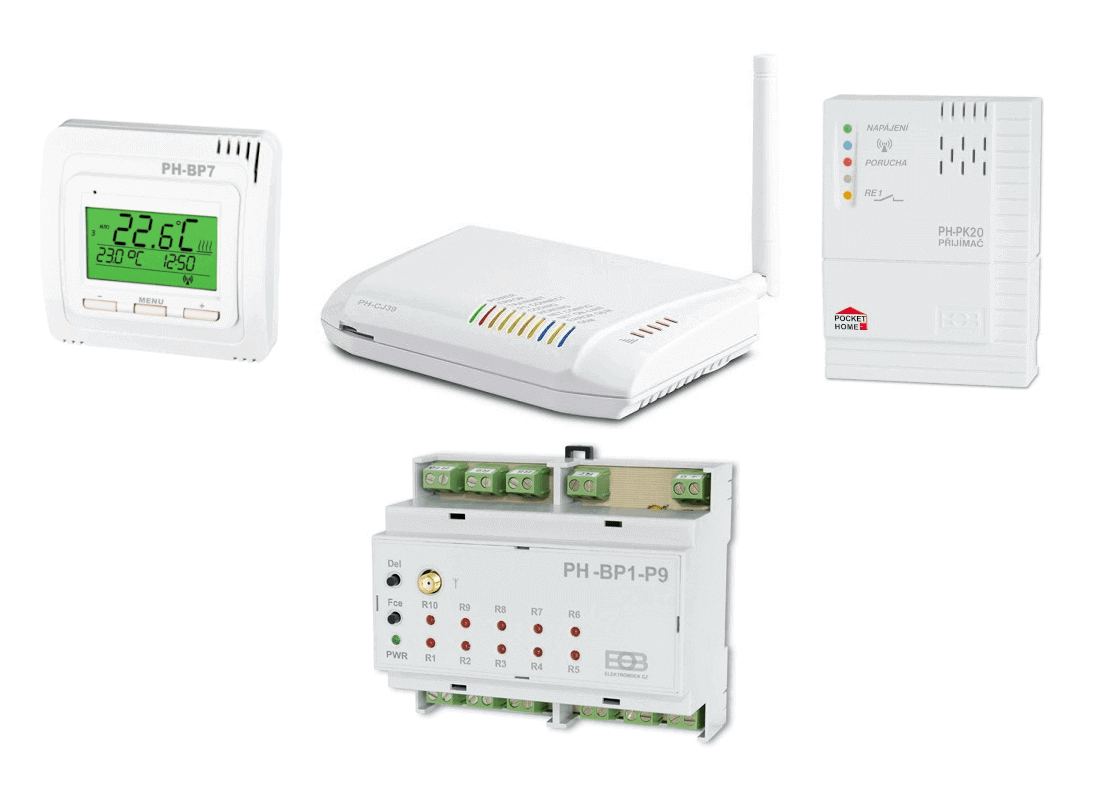
\includegraphics[width=\textwidth]{images/komercni-systemy/elektrobock-pocket-home/elektrobock-pocket-home.png}}
\put(50,226){\scriptsize \sffamily a)}
\put(180,190){\scriptsize \sffamily b)}
\put(305,235){\scriptsize \sffamily c)}
\put(180,8){\scriptsize \sffamily d)}
	 \caption{Jednotlivá zařízení systému Elektrobock PocketHome. a) Nástěnný snímač prostorové teploty. b) Centrální jednotka. c) Spínací jednotka kotle. d) Zónový regulátor. Upraveno z \cite{elektrobock-lokalni-termostat, elektrobock-centralni-jednotka, elektrobock-spinaci-jednotka-kotle, elektrobock-zonovy-regulator}.}
	 \label{fig:elektrobock-pocket-home}
\end{picture}

\end{figure}

\subsection{Honeywell}
Honeywell nabízí bezdrátový systém regulace podlahové topení. Systém řízení je zastřešené pod aplikaci Evohome. Skládá se z centrální jednotky s~dotykovým displejem, nástěnných snímačů prostorové teploty pro jednotlivé místnosti, zónového regulátoru pro ovládání jednotlivých topných okruhů (celkově je možné ovládat 5 zón, s rozšiřovacím modulem je možné se dostat na 8 zón). Systém je možné rozšířit o dobíjení TUV, pro sledování teploty na zásobníku je možné umístit teplotní čidlo, ze kterého je teplota odesílaná do centrální jednotky. Na obrázku \ref{fig:honeywell-evohome} jsou zobrazeny jednotlivé zařízení systému. Systém však při dobíjení zásobníku TUV počítá se zdrojem tepla pouze s kotlem, takže v případě využití krbů s výměníkem nastává problém. V neposlední řadě umožňuje zapojit směšovací ventil pro optimální teplotu do podlahového topení. Systém je možné ovládat lokálně nebo řídit vzdáleně odkudkoliv, je zapotřebí se zaregistrovat si účet a spárovat ho s  centrální jednotkou. Vzdálený server přijímá požadavky na změny režimů či nastavení teplot, a zasílá je do řídící jednotky. Server průběžně shromažďuje různá data o chování soustavy, a může je na základě žádosti poskytnout. Z toho vyplývá, že pro lepší řízení a nastavení vytápění je nutné zřídit vzdálený přístup a samotné vyhodnocení a dání povelů, pak dochází na vzdálením serveru, nemáme moc pod kontrolou data a životnost takového systému do budoucnosti. Otázka je i při využití pouze lokálního režimu, zda regulace nepřichází o výhody cloudového řešení. Problém bezdrátového řešení může být opět prostup signálu mezi zařízeními a centrální jednotkou (popsaný u předešlého systému), zejména prostup železobetonovými podlahami a to především při komunikace mezi centrální jednotkou umístěnou v patře a~komunikací mezi se zařízeními ve sklepě (nutný průchod dvěma podlahami) a je nutná výměna baterií v zařízeních po určité době. Komunikace mezi zařízeními probíhá na frekvenci 868 MHz, připojení k centrální jednotce pomocí mobilní aplikace je pomocí WiFi (respektive centrální jednotka je připojena na domácí WiFi router, komunikace pak probíhá mezi aplikací, vzdáleným serverem a~centrální jednotkou).

\begin{figure}[H]

\centering
\begin{picture}(370,300)
\put(0,0){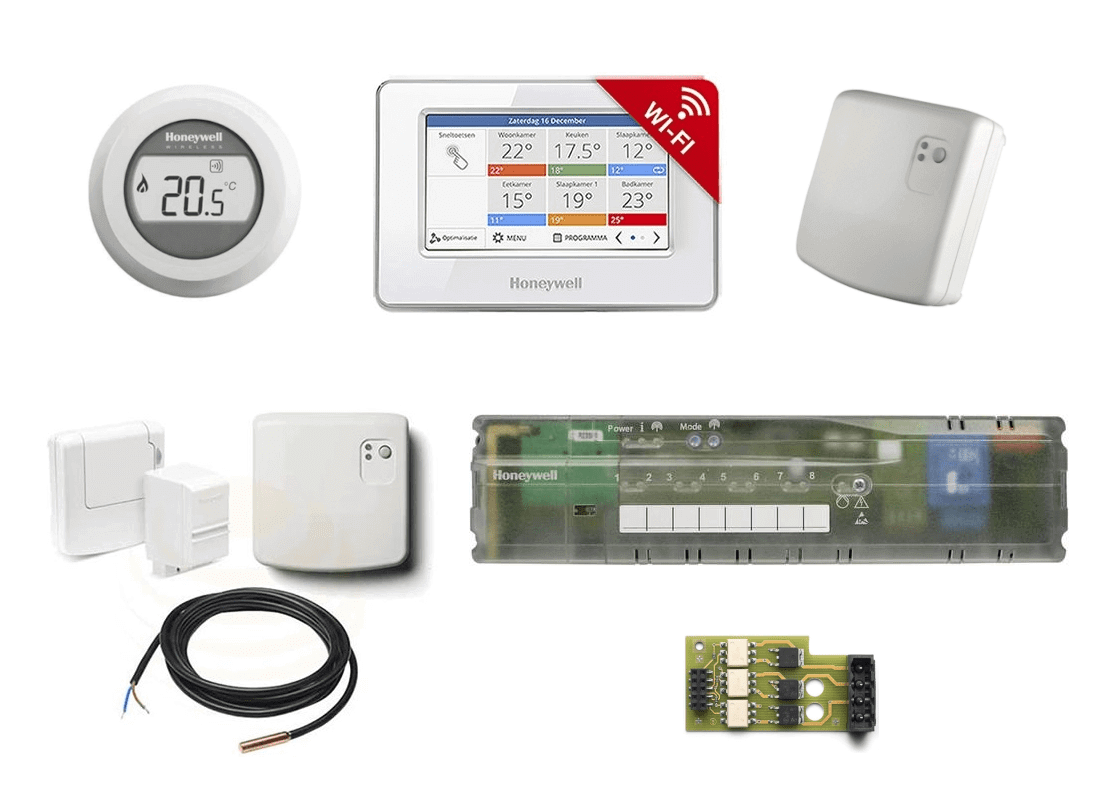
\includegraphics[width=\textwidth]{images/komercni-systemy/honeywell-evohome/honeywell-evohome.png}}
\put(60,240){\scriptsize \sffamily a)}
\put(180,240){\scriptsize \sffamily b)}
\put(305,240){\scriptsize \sffamily c)}
\put(60,130){\scriptsize \sffamily d)}
\put(250,130){\scriptsize \sffamily e)}
\put(250,57){\scriptsize \sffamily f)}
	 \caption{Jednotlivá zařízení systému Honeywell Evohome. a) Nástěnný snímač prostorové teploty. b) Centrální jednotka. c) Spínací jednotka kotle. d) Řízení dobíjení TUV. e) Zónový regulátor. f) Rozšiřující modul pro  zónový regulátor. Upraveno z \cite{honeywell-lokalni-termostat, honeywell-centralni-jednotka, honeywell-spinaci-jednotka-kotle, honeywell-rizeni-dobijeni-tuv, honeywell-zonovy-regulator, honeywell-rozsirujici-modul-pro-zonovy-regulator}.}
	 \label{fig:honeywell-evohome}
\end{picture}

\end{figure}

\subsection{Danfoss}
Danfoss nabízí bezdrátový systém regulace podlahové topení. Systém řízení je zastřešené pod aplikaci Danfoss Link.  Řídící systém se skládá z centrální jednotky s dotykovým displejem, nástěnných snímač prostorové teploty  pro jednotlivé místnosti a zónového regulátoru pro ovládání jednotlivých topných okruhů (celkově je možné ovládat 10 zón), oběhového čerpadla a řízení kotle. Na obrázku \ref{fig:danfoss-danfoss-link} jsou zobrazeny jednotlivé zařízení systému. Obdobným problém jako u PocketHome je počítání pouze s jedním zdrojem tepla, nepočítání s centrálním zásobníkem teplé vody. Vzdálené ovládání umožněno přes mobilní aplikací pomocí cloudové řešení. Systém má absenci v řízení dobíjení TUV, respektive zásobníku na otopnou vodu a použít více zdrojů tepla (viz předchozích systémy). Opětovnými problémy může být šíření bezdrátového signálu mezi zařízeními (výrobce nabízí zesilovače/opakovače pro signál), problémy cloudového řešení a nutná výměna baterií po určité době (problémy více popsány u předešlých systémů). Komunikace mezi zařízeními probíhá na frekvenci 868 MHz, připojení k centrální jednotce je možné pomocí mobilní aplikace.

\begin{figure}[h]
\centering
\begin{picture}(370,180)
\put(0,0){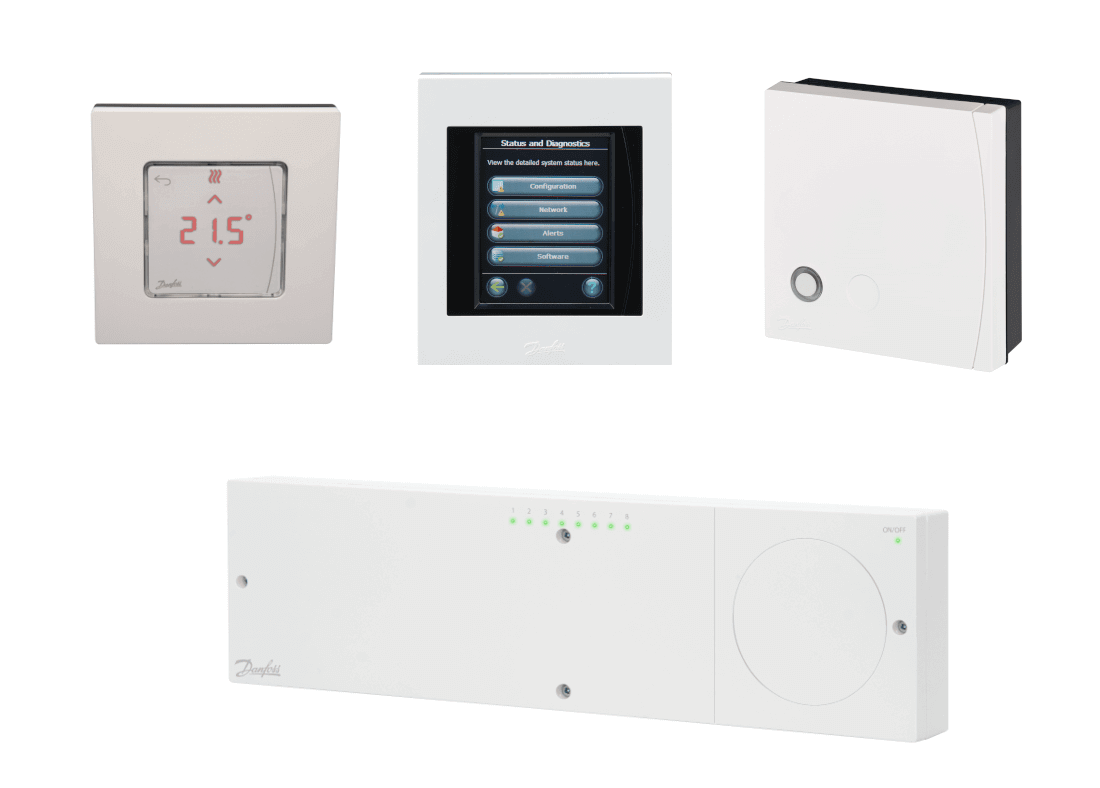
\includegraphics[width=\textwidth]{images/komercni-systemy/danfoss-danfoss-link/danfoss-danfoss-link.png}}
\put(60,242){\scriptsize \sffamily a)}
\put(180,242){\scriptsize \sffamily b)}
\put(305,242){\scriptsize \sffamily c)}
\put(180,102){\scriptsize \sffamily d)}
	 \caption{Jednotlivá zařízení systému Danfoss Danfoss Link. a) Nástěnný snímač prostorové teploty. b) Centrální jednotka. c) Spínací jednotka kotle. d) Zónový regulátor. Upraveno z \cite{danfoss-lokalni-termostat, danfoss-centralni-jednotka, danfoss-zonovy-regulator, danfoss-spinaci-jednotka-kotle}.}
	 \label{fig:danfoss-danfoss-link}
\end{picture}

\end{figure}

Pokud shrnu hlavní nedostatky zmíněných systému pro řízení podlahové vytápění, tak mezi ně patří bezdrátové ovládání, zejména tedy možný problém komunikace mezi centrální jednotkou a zařízeními, výměna baterií po určité době. Dále absence počítání s více zdroji tepla a s centrálním zásobníkem otopné vody, systém od firmy Honeywell počítá alespoň s ohřevem TUV. Další možným nedostatkem může být cloudové řešení z pohledu dlouhodobé garance fungování služby, další věcí pak je že vzdálené ovládání neprobíhá přímo s centrální jednotkou, ale se vzdáleným serverem. Další zjištěním bylo, že všechny systémy jsou nabízeny jako bezdrátové, což je samozřejmě pochopitelné jak z pohledu jednoduchého nainstalování, již do stávajících obydlí, kde s takovým to systémem nebylo počítáno (zejména staré zástavby), též není nutné provádět žádné stavební úpravy. Pokud jsou nabízené drátové řešení, tak zde není žádná centrální jednotka, ovládání probíhá přes drátové lokální termostaty připojené přímo na zónový regulátor, který následně ovládá jednotlivé topné okruhy. Tabulka \ref{tab:srovnani-vlastnosti-jednotlivych-komercnich-systemu} zobrazuje přehled možností systémů zmíněné výše.


\begin{center}
\begin{table}[H]
\begin{threeparttable}
\begin{tabular}{|c||c|c|c|} \hline
\backslashbox{Funkce}{Systém}
& \thead{Elektrobock \\ (PocketHome)}  & \thead{Honeywell \\ (Evohome)} & \thead{Danfoss \\ (Danfoss Link)} \\


\hline
\thead{Napojení na více \\ zdrojů tepla} & Ne & Ne & Ne \\ 
\hline
\thead{Napojení na \\ centrální zásobník \\ topné vody} & \multirow{2}{*}{Ne} & \multirow{2}{*}{Ne} & \multirow{2}{*}{Ne} \\ 
\hline
\thead{Ohřev TUV} & Ne & Ano & Ne \\ 
\hline
\thead{Bezdrátové$\slash$drátové \\ řešení} & Ano & Ano & Ano \\ 
\hline
\thead{Možnosti ovládání} & \makecell{PC \\ chytrý telefon} & \makecell{dotykový displej \\ chytrý telefon } & chytrý telefon \\ 
\hline
\thead{Cloudové řešení} & Ne & Ano & Ano \\ 
\hline
\makecell{Centrální \\ řídicí jednotka} & \makecell{(PH-CJ39-WIFI, 1×) \\ 3 678 Kč}  & \makecell{(ATC928G3026,  1×) \\ 5 994 Kč } & \makecell{(014G0288, 1×) \\ 8 694 Kč }\\
Zónový regulátor & \makecell{(PH-BP1-P9, 1×) \\ 3 388 Kč} & \makecell{(HCE80, 1×) \\ 5 622 Kč} & \makecell{(088U1031, 1×) \\ 4 299 Kč} \\
\makecell{Nástěnný snímač \\ prostorové teploty} & \makecell{(PH-BP7-V, 9×) \\ 9 036 Kč} & \makecell{(T87RF2083, 9×) \\ 12 141 Kč} & \makecell{(088U1081, 9×) \\ 19 476 Kč} \\
Spínací jednotka kotle & \makecell{(PH-PK20, 1×) \\ 1 498 Kč} & \makecell{(BDR91A1000, 1×) \\ 1 100 Kč} & \makecell{(014G0272, 1×) \\ 2 190 Kč}\\
Řízení dobíjení TUV & & \makecell{(ATF500DHW, 1×) \\ 3 818 K}  & \\
\makecell{Rozšiřující modul \\ pro zónový regulátor}  & & \makecell{(HCS80, 1×) \\ 1 897 Kč} & \\
\thead{Celková cena \\ včetně DPH \tnote{a}} & 17 600 Kč & 30 572 Kč & 34 659 Kč\\ 
\hline
\end{tabular}

	\begin{tablenotes}
    	\item[a] Ceny stanoveny ke dni 26. 11. 2020.
	\end{tablenotes}

\end{threeparttable}

	 \label{tab:srovnani-vlastnosti-jednotlivych-komercnich-systemu}
 \caption{Srovnání funkcí jednotlivých komerčních systémů.}
\end{table}
\end{center}

V tabulce \ref{tab:srovnani-vlastnosti-jednotlivych-komercnich-systemu} chybí v části ceny pohony pro ovládání jednotlivých topných okruhů pomocí zónového regulátoru. Pro výše zmíněné systémy, zónový regulátor podporuje pohony na 230 V AC, pohony je možné koupit  přímo od daného výrobce nebo od jiného, na samotnou funkčnost to nemá vliv. Jediný rozdíl může být v pořizovací ceně, kde pro termoelektrické pohony je cena od 400 do 800 Kč, pro servopohony může být cena ještě vyšší. Celková cena za 12 pohonů se pohybuje v řádu jednotek tisíc. Někteří výrobci jako Danfoss nabízejí pro jejich systém zesilovače/opakovače signálu pro bezdrátový systém, v případě špatného průchodu signálu je možné zakoupit toto zařízení, ale nutné počítat s dalšími náklady na víc (řády jednotek tisíc). V případě, že systém neumí ovládat kotel pro dobíjení TUV, případně nesplňuje požadavky, které bychom chtěli, pak je nutné využít jiné řešení/systém, což se dále promítá do dalších nákladů a hlavně se jedná o nejednotnost jednoho systému.







